\documentclass{beamer}

\usepackage{préambule}

\begin{document}
\small

\newcommand{\Exercice}{
	\begin{frame}
		ABCDEFGH est un octogone régulier de centre O. 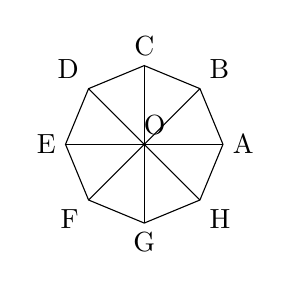
\begin{tikzpicture}
			\coordinate (O) at (0,0);
			\coordinate (A) at (1,0);
			\coordinate[rotate around={45:(O)}] (B) at (A);
			\coordinate[rotate around={45:(O)}] (C) at (B);
			\coordinate[rotate around={45:(O)}] (D) at (C);
			\coordinate[rotate around={45:(O)}] (E) at (D);
			\coordinate[rotate around={45:(O)}] (F) at (E);
			\coordinate[rotate around={45:(O)}] (G) at (F);
			\coordinate[rotate around={45:(O)}] (H) at (G);

			\draw (A) -- (B) -- (C) -- (D) -- (E) -- (F) -- (G) -- (H) -- (A);
			\node[above right,xshift=-0.13cm] at (O) {O};
			\foreach \p/\dir in {A/right,B/above right,C/above,D/above left,E/left,F/below left,G/below,H/below right} {
					\node[\dir] at (\p) {\p};
					\draw (O) -- (\p);
				}
		\end{tikzpicture}

		\begin{enumerate}
			\item Compléter le tableau suivant par oui ou non :

			      \hspace*{-1cm}\begin{tabular}{|l|c|c|c|c|}
				      \hline
				      Les vecteurs          & $\vec{GH}$ et $\vec{BC}$ & $\vec{AE}$ et $\vec{BD}$ & $\vec{FD}$ et $\vec{HB}$ & $\vec{AH}$ et $\vec{ED}$ \\ \hline
				      ont la même direction & \correction{non}         & \correction{oui}         & \correction{oui}         & \correction{oui}         \\ \hline
				      ont le même sens      & \correction{non}         & \correction{oui}         & \correction{oui}         & \correction{non}         \\ \hline
				      ont la même norme     & \correction{non}         & \correction{non}         & \correction{oui}         & \correction{oui}         \\ \hline
				      sont opposés          & \correction{non}         & \correction{non}         & \correction{non}         & \correction{oui}         \\ \hline
			      \end{tabular}
			\item Indiquer à chaque fois si l'affirmation est vraie ou fausse :
			      \begin{multicols}{2}
				      \begin{itemize}
					      \item $\vec{GH}$ et $\vec{OB}$ sont égaux : \correction{FAUX}
					      \item $\vec{FE}$ et $\vec{BA}$ sont opposés : \correction{VRAI}
					      \item $\vec{GF}$ et $\vec{OE}$ sont opposés : \correction{FAUX}
					      \item $\vec{AF}$ et $\vec{DC}$ sont égaux : \correction{FAUX}
				      \end{itemize}
			      \end{multicols}
		\end{enumerate}
	\end{frame}
}

\Exercice

\newcommand{\makeCorrection}{}
\Exercice

\end{document}